\documentclass[12pt]{article}
\usepackage{amsfonts, amsmath, amsthm, amssymb}
\usepackage[left=1cm,right=1cm,top=1cm,bottom=2cm]{geometry}
\usepackage{paralist}
\usepackage[T2A]{fontenc}
\usepackage[russian]{babel}
\usepackage[utf8]{inputenc}
\usepackage{graphicx}
\usepackage{wrapfig}

\usepackage{mathtools}
\usepackage{comment}

\newcounter{problem}
\newcommand{\problem}{\par \bigskip \refstepcounter{problem}%
\textbf{№\arabic{problem}.} }

\def \Problem#1{\par \bigskip \textbf{Задача №{#1}. }}
\def \solution{\par \bigskip \textbf{Решение. }}
\def \solutionI{\par \bigskip \textbf{Первое решение. }}
\def \solutionII{\par \bigskip \textbf{Второе решение. }}
\def \solutionIII{\par \bigskip \textbf{Третье решение. }}
\def \Lemma{\par \bigskip \textbf{Лемма. }}
\def \lemma#1{\par \bigskip \textbf{Лемма {#1}. }}
\def \proof{\par \bigskip \textbf{Доказательство. }}
\def \answer{\par \bigskip \textbf{Ответ. }}
\def \marking{\par \bigskip \textbf{Схема оценки. }}
\def\geq{\geqslant}
\def\leq{\leqslant}
\def\frac#1#2{\mathchoice{#1\over#2}{\hbox{\small$#1$}\over\mathstrut\hbox{\small$#2$}}{#1\over#2}{#1\over#2}} 

\begin{document}
\centerline{\sc \textbf{XXI Математическая олимпиада "Шелковый путь"}}

\centerline{\sc \textbf{Март 2022 года}}

\bigskip
\hrule
\bigskip

\textsl{\textbf{Внимание!} 
Так как XXI Математическая олимпиада «Шелковый путь» проводится в Казахстане
раньше, чем в других странах, мы Вас убедительно просим \textbf{не разглашать}
эти задачи и не обсуждать их (особенно по Интернету) до 25 мая 2022 года.}

\bigskip

\centerline{\sc \textbf{Решения задач и схемы оценивания}}

\bigskip
\Problem{1} В окружность $\omega$ вписан выпуклый четырехугольник $ABCD$. Лучи $AB$ и $DC$ пересекаются в точке $K$. На диагонали $BD$ отмечена точка $L$ так, что $\angle BAC = \angle DAL$. На отрезке $KL$ отметили точку $M$ так, что $CM \parallel BD$. Докажите, что прямая $BM$ касается окружности $\omega$. \textit{(Кунгожин~М.)}

\begin{wrapfigure}{r}{0.3\textwidth}
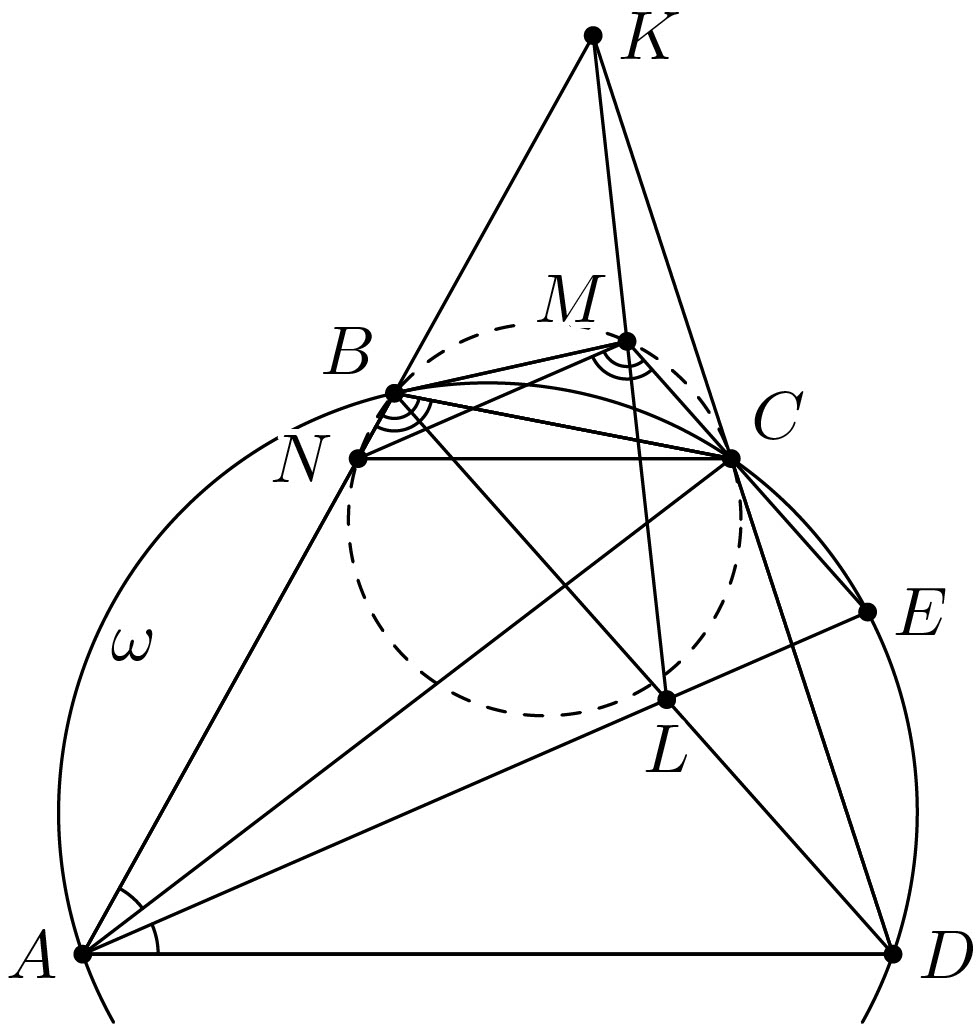
\includegraphics[width=0.3\textwidth]{img_1.jpg}
\end{wrapfigure}
\solutionI Отметим на прямой $AK$ точку $N$ такую, что $MN \parallel AL$. Тогда точка $K$ является центром гомотетии, переводящей треугольник $CMN$ в подобный ему треугольник $DLA$, так как $\frac{CM}{DL}=\frac{NM}{AL}=\frac{KM}{KL}$ и $\angle CMN=\angle DLA$. Но, с другой стороны, треугольник $DLA$ подобен треугольнику $CBA$, так как $\angle DAL=\angle BAC$ и $\angle ADL = \angle ACB$. Следовательно, $\angle(BN, BC)=\angle(MN,MC)$, то есть точки $N,B,M,C$ лежат на одной окружности. Поэтому, $\angle CBM=\angle CNM=\angle CAB$. Из последнего равенства следует, что $BM$ касается~$\omega$.

\solutionII Для этого решения нам понадобится следующая теорема.

\textbf{Теорема Паскаля.} Точки $A$, $B$, $C$, $D$, $E$, $F$ лежат (не обязательно в этом порядке) на одной окружности. Тогда точки пересечения прямых $AB$ и $DE$, $BC$ и $EF$, $CD$ и $FA$ лежат на одной прямой.

Вернемся к решению задачи. Пусть прямая $AL$ пересекает $\omega$ во второй раз в точке $E$. Тогда точки $M$, $C$, $E$ лежат на одной прямой, так как $\angle MCK=\angle LDC=\angle BAC=\angle DAE=\angle DCE$.

Обозначим через $\ell_b$ касательную  прямую к $\omega$ в точке $B$. Применим теорему Паскаля для точек $B$, $B_1$, $A$, $E$, $C$, $D$ (здесь точка $B_1$ совпадает с точкой $B$) и для пар прямых $(BB_1,EC)$, $(B_1A,CD)$, $(AE,DB)$. Последние пары прямых определяют соответственно пары $(\ell_b, EC)$, $(BA,CD)$, $(AE, DB)$. Тогда по теореме Паскаля, на прямой, соединяющей точки $K=BA\cap CD$, $L=AE\cap DB$, лежит точка пересечения прямых $\ell_b$ и $EC$. Но так как $M=EC \cap KL$, то $BM$ касается окружности $\omega$. 

\marking
\\ 1. Недоведенное счетное решение \\(в координатах, в комплексных числах, в векторах, тригонометрическое, и т.д.): \dotfill \textbf{0 баллов}
\\ 2. Доказано подобие $\triangle ADL \sim \triangle ACB$ (с указанимем этих двух треугольников): \dotfill \textbf{1 балл} 
\\ 3. Доказано подобие $\triangle CMN \sim \triangle DLA$: \dotfill \textbf{3 балла}
\\ 4. Доказано (с выводом), что точки $N,B,M,C$ лежат на одной окружности: \dotfill \textbf{2 балла}
\\ 5. Доказано, что точки $M,C,E$ лежат на одной прямой: \dotfill \textbf{1 балл}
\\ Не суммируется с пунктом 2.
\\ 6. Применение т. Паскаля без никаких деталей (относительно того, к чему ее применять): \dotfill \textbf{0 баллов}
\\ 7. Теорема Паскаля применена к неправильной шестерке точек: \dotfill \textbf{0 баллов}
\\ 8. Указана правильная шестерка точек к которым применяется т. Паскаля, но порядок точек в шестиугольнике не дан либо указан в неправильном порядке: \dotfill \textbf{минус 2 балла}
\\ 9. За нерассмотрение всевозможных расположений точек баллы не снимаются.


\Problem{2} Даны два различных натуральных числа $A$ и $B$. Докажите, что существует бесконечно много натуральных чисел, представимых и в виде $x_1^2+Ay_1^2$ со взаимно простыми $x_1$ и $y_1$, и в виде $x_2^2+ By_2^2$ со взаимно простыми $x_2$ и $y_2$.
\textit{(Голованов А.С.)}

\solution  Не теряя общности, пусть $A>B$.

Возьмём произвольное простое $p>2$ и подберём такие
$x_1$, $x_2$, что
$$x_1^2+A(2p)^2=x_2^2+B(2p)^2,$$
то есть $x_2^2-x_1^2=4Cp^2$, где $C=A-B$. Этому уравнению удовлетворяют
$x_1=Cp^2-1$ и $x_2=Cp^2+1$. Если полученные $x_1$ и $x_2$ нечётны, они взаимно
просты с $y=2p$, и $x_1^2+Ay^2=x_2^2+By^2$. Если же они чётны, то
$\frac{x_1}{2}$ и $\frac{x_2}{2}$ взаимно просты с $p$,
и $\left(\frac{x_1}{2}\right)^2+Ap^2=\left(\frac{x_2}{2}\right)^2+Bp^2$.

Осталось заметить, что число, для которого таким образом получены два
искомых представления, во всяком случае не меньше $p^2$, и поэтому может
быть сколь угодно большим.

\marking
\\ 1. Доказано, что если $x_1 = Cp^2 - 1$ и $x_2 = Cp^2 + 1$ оба нечётны, то число $x_1^2 + Ay^2 = x_2^2 + By^2$ удовлетворяет условию задачи, где $y = 2p$ : \dotfill \textbf{ 5 баллов} 
\\ 2. Доказано, что если $x_1 = Cp^2 - 1$ и $x_2 = Cp^2 + 1$ оба чётны, то число $\left(\frac{x_1}{2}\right)^2+Ay^2=\left(\frac{x_2}{2}\right)^2+By^2$ удовлетворяет условию задачи, где $y = p$: \dotfill \textbf{ 5 баллов} 
\\ 3. Показано, что таких чисел бесконечно (при наличии одного из пунктов 1 или 2): \dotfill \textbf{ 1 балл}
\\ 4. Баллы за 1. и 2. не суммируются: \dotfill
\\ 5. При наличии 1. и 2. одновременно: \dotfill \textbf{плюс 1 балл}

\Problem{3} В бесконечной последовательности $\{\alpha\}$, $\{\alpha^2\}$, $\{\alpha^3\}$, \dots  встречается только конечное количество разных чисел. Докажите, что $\alpha$ -- целое. (Дробной частью числа $x$ называется такое число~$\{x\}$, что $\{x\} = x-[x]$, где $[x]$ это наибольшее целое число, не превосходящее $x$.) \textit{(Голованов А.С.)}

\solution \textit{Шаг 1.} Предположим, что в последовательности всего встречается 
$k-1$ число. Для каждого натурального $n$ среди чисел $\{\alpha^{nk}\}$, 
$\{\alpha^{nk+1}\}$, \dots, $\{\alpha^{nk+k-1}\}$ найдутся два одинаковых. 
Таким образом, существует бесконечно много пар натуральных чисел $i$, $j$, 
$0<i-j<k$, для которых $\{\alpha^i\}=\{\alpha^j\}$, то есть 
$\alpha^j(\alpha^{i-j}-1)$ -- целое число. Поскольку во всех таких парах 
$i-j$ принимает конечное число значений, следовательно, хотя бы одно из этих 
значений принимается бесконечно много раз. Таким образом, нашлось некоторое 
$m$ такое, что $\alpha^j(\alpha^m-1)$ целое для бесконечно многих $j$. 
Деля полученные числа друг на друга, находим, что их частные рациональны. 
Эти частные -- степени $\alpha$ с натуральным показателем. Итак, $\alpha^l$ 
рационально для некоторого натурального $l$. 

   \textit{Шаг 2.} Если $\alpha^l$ -- не целое, а представляется несократимой дробью $a\over b$ 
с натуральным знаменателем $b>1$, то $\{\alpha^{ln}\}$ -- несократимая дробь 
со знаменателем $b^n$. Так как при всех натуральных $n$ такие знаменатели различны, 
получаем противоречие с условием. Итак, $\alpha^l$ -- целое число. 
Если при этом $\alpha$ иррационально, то числа вида 
$\alpha^{nl+1}=\alpha^{nl}\cdot \alpha$ при всех натуральных $n$ иррациональны 
и имеют различные дробные части (ибо число 
$\alpha^{il+1}-\alpha^{jl+1}=\alpha (\alpha^{il}-\alpha^{jl})$, как 
произведение иррационального $\alpha$ и целого числа, отличного от 0, не может 
быть целым). Это тоже противоречит условию. Таким образом, $\alpha$ 
рационально. Как известно, при целом $\alpha^l$ отсюда следует, что $\alpha$ 
целое, что и требовалось. 

\marking
\\ 1. Доказательство шага 1: \dotfill \textbf{4 балла}
\\ 2. Попытка построения $m$ такого, что $\alpha^j(\alpha^m-1)$ --- целое для двух различных $j$: \dotfill \textbf{1 балл}
\\ 3. Найдены $i$, $j$ такие, что $\{\alpha^i\}=\{\alpha^j\}$ и $|i-j|$ ограничен сверху константой, которая может зависеть от $k$ (но не от $i$, $j$): \dotfill \textbf{2 балла}
\\ 4. Доказательство шага 2, т.е. что если $\alpha^l$ --- рационально, то $\alpha$ --- целое: \dotfill \textbf{2 балла}
\\ 5. Доказательство того, что если $\alpha$ рационально, то $\alpha$ --- целое: \dotfill \textbf{1 балл}
\\ 6. Пункт 1 не складывается с пунктами 2 и 3, пункт 4 не складывается с пунктом 5.

\Problem{4} В письменности используется 25-буквенный алфавит, а \emph{словами} являются в точности все 17-буквенные последовательности. На полоске, склеенной в кольцо, написана последовательность из $5^{18}$ букв алфавита. Назовём слово \emph{уникальным}, если из полоски можно вырезать участок, содержащий это слово, но нельзя вырезать два таких непересекающихся участка. Известно, что из полоски можно вырезать $5^{16}$ непересекающихся копий какого-то слова. Найдите наибольшее возможное количество уникальных слов.  \textit{(Богданов И.)}

\answer $2\cdot 5^{17}$.
\solution Пусть алфавит состоит из букв $a_1,a_2,\dots,a_{25}$. Назовём \emph{куском} участок полоски, содержащий ровно 17 букв (разные куски могут содержать одинаковые слова!). Кусок назовём \emph{уникальным}, если слово, написанное на нём, уникально.

\medskip
Построим сначала пример, в котором найдётся $N=2\cdot 5^{17}$ уникальных слов. Выберем слово $W=a_1a_2\dots a_{17}$ --- это будет слово, повторяющееся $k=5^{16}$ раз. Существует всего $25^8=k$ восьмибуквенных последовательностей, состоящих из букв $a_{18}, a_{19}, \ldots, a_{25}$; выпишем их всех на полоску в произвольном порядке, приписав после каждой слово $W$. Назовём $5^{16}$ участков полоски, содержащих выписанные восьмибуквенные последовательности, \emph{фрагментами}. Мы выписали $(8+17)k=5^{18}$ букв,

Ясно, что полученная полоска содержит $k$ копий слова $W$. Покажем, что любой кусок, содержащий целиком некоторый фрагмент, уникален --- более того, слово на нём не встречается на других кусках. Поскольку фрагмент может располагаться в таком куске на 10 различных позициях (начинаясь с первой, второй, \dots, или десятой буквы слова), таких уникальных слов получится как раз $10 k = 10\cdot 5^{16}=N$.

\smallskip
Рассмотрим произвольный кусок $p$ и слово $P$, написанное на нём. У этого слова либо есть единственное непустое начало, являющееся концом $W$, либо такого начала нет --- ровно в этом случае будем считать, что начало пустое. Обозначим длину этого начала через $b$. Аналогично определим конец слова $P$, являющийся началом $W$,  и его длину $e$. Заметим, что эти начало и конец не перекрываются (в случае, когда $P\neq W$, иначе $b=e=17$).

Если кусок не содержит фрагмента, то $\max\{b,e\}>9$. Если наш кусок содержит фрагмент, то $b+e=9$ и $0 \le b, e \le 9$. Итак, кусок $p$ содержит фрагмент ровно тогда, когда $\max\{b,e\}\leq 9$, и при этом положение в нём фрагмента (а значит, и положение такого куска на полоске) восстанавливается однозначно. Значит, любой такой кусок уникален, и построенный пример подходит.

\medskip
Осталось доказать, что уникальных слов не может быть больше, чем $N$. Пронумеруем позиции на полоске последовательно числами $1,2,\dots,5^{18}$ (нумерация циклическая по модулю $5^{18}$). Пусть  $p_i$ --- кусок, начинающийся с позиции $i$, а $P_i$ --- слово на нём. Пусть $n_1,\dots,n_k$ --- позиции такие, что куски $p_{n_1}$, $p_{n_2}$, \dots, $p_{n_k}$ попарно не перекрываются и содержат одно и то же слово $W$ из условия. Эти куски, очевидно, не уникальны.

При $i=1,2,\dots,8$ назовём \emph{последователем $i$-го ранга} кусок вида $p_{n_s+i}$, а \emph{предшественником $i$-го ранга} --- кусок вида $p_{n_s-i}$, где $1\leq s\leq k$. Все определённые куски различны, причём все последователи одного ранга не перекрываются, то же верно для предшественников. Мы покажем, что \textit{среди $8\cdot 5^{16}$ последователей всех рангов не более $5^{16}$ уникальных кусков}; из симметрии, то же будет выполняться и для предшественников. Из этого будет следовать, что есть не менее $5^{16}+7\cdot 5^{16}+7\cdot 5^{16}=3\cdot 5^{17}$ неуникальных кусков, откуда и следует требуемая оценка.

\smallskip
Итак, осталось доказать выделенное утверждение про последователей. В каждом последователе $p_{n_s+i}$ ранга $i$ выделим его \emph{хвост} %$T_{s,i}$ 
--- конец длины $i$ (он состоит ровно из букв, не вошедших в $p_{n_s}$). Докажем индукцией по $m=0,1,\dots,8$, что для любой $(8-m)$-буквенной последовательности $U$, уникальных последователей, хвосты которых начинаются c последовательности~$U$, не больше, чем $25^m$. Тогда при $m=8$ получим, что всего уникальных последователей не более, чем $25^8=k$, что и требовалось.

База при $m=0$ очевидна: если последователь с 8-буквенным хвостом $U$ уникален, то такой последователь лишь один. Докажем переход. Если нет уникального последователя, хвост которого --- это $U$, то все хвосты уникальных последователей,  начинающимися на $U$, на самом деле начинаются на некоторую последовательность $Ua_j$. При каждом из 25 возможных значений $j$ таких уникальных последователей не больше, чем $25^{m-1}$ по предположению индукции, поэтому всего их не больше $25\cdot 25^{m-1}=25^m$, что и требовалось.

Наконец, если есть уникальный последователь $P_{n_s+8-m}$, хвост которого есть $U$, то такой последователь единственен. Поэтому все последователи б\'{о}льших рангов, хвосты которых начинаются на $U$, соответствуют той же копии $p_{n_s}$ слова $W$. Поэтому всего таких уникальных последователей не больше $m+1\leq 25^m$, что, опять же, и требовалось. Утверждение, а вместе с ним и оценка, доказаны.

\medskip
\textbf{Замечание.} Более коротко (но и более идейно!) выделенное курсивом утверждение можно доказать так. Назовём хвост $T$ уникального последователя \emph{минимальным}, если никакое его начало не является хвостом уникального последователя. В частности, никакой минимальный хвост не является началом другого минимального хвоста.

Для каждого минимального хвоста $T$ выпишем все 8-буквенные последовательности, начинающиеся на $T$; если длина $T$ равна $d$, то мы выписали $25^{8-d}$ последовательностей. Никакая последовательность не выписана дважды; значит, если есть всего $M$ минимальных хвостов длин $d_1,\dots,d_M$, то
$$
  \sum_{i=1}^M 25^{8-d_i}\leq 25^8.
$$

С другой стороны, каждый хвост уникального последователя начинается с минимального хвоста. Для минимального хвоста $T$ длины $d$ таких последователей может быть лишь $9-d$ --- по одному для каждой длины хвоста. Значит, общее количество уникальных последователей не превосходит
$$
  \sum_{i=1}^M (9-d_i)\leq \sum_{i=1}^M 25^{8-d_i}\leq 25^8,
$$
поскольку $9-d\leq 25^{8-d}$ при всех $d=1,2,\dots,8$.

\marking
\\ 1. Пример с $2\cdot 5^{17}$ уникальными словами: \dotfill \textbf{2 балла}
\\ 2. Доказательство корректности примера: \dotfill \textbf{1 балл}
\\ 3. Доказательство того, что ответ не больше $2\cdot 5^{17}$: \dotfill \textbf{4 балла}
\\ 4. Формулировка выделенного курсивом утверждения: \dotfill \textbf{1 балл}
\\ 5. Баллы за 3. и 4. не складываются.

\end{document}
